\newpage
\title{LEZIONE 12 30/03/2020}\newline
\textbf{link} \href{https://web.microsoftstream.com/video/05bd4cd5-c99f-4a6c-9334-733e9a60083a?list=user&userId=faa91214-a6f5-40d7-8875-253fd49b8ce1}{clicca qui}
\section{Risposta esponenziale (SD LTI a TC, SISO)}
\subsection{Domanda}
Dato il sistema $\begin{cases}
    \dot{x} = Ax +bu\\ y = cx +du
\end{cases}$ sottoposto all'ingresso $u(t) = e^{\lambda t}$ con $t\geq 0$ (o equivalentemente $e^{\lambda t} sca(t)$), esiste uno stato iniziale $x(0)$ tale che $x(0)$ e $u(t)$ producono un'uscita $y(t)= Y e^{\lambda t}$, con $Y$ un numero qualunque (non la trasformata) e $t \geq 0$?\newline
\newline
In altri termini:\newline
Sottoponiamo un sistema dinamico (di cui non sono note le proprietà sulla sua stabilità) a un ingresso esponenziale ($u(t) = e^{\lambda t}$, che può anche essere amplificato come $u(t) = U e^{\lambda t}$, ovviamente il ragionamento non cambia). Detto questo sappiamo che un ingresso $x(0)$ produce un movimento libero di $y$ fatto da modi, invece un uscita del tipo $u(t) = e^{\lambda t}$ produce un movimento forzato fatto da modi $+$ un termine $Ye^{\lambda t}$ (con $t \geq 0$ e con $Y$ un numero, non la trasformata). La domanda è se esiste uno $x(0)$ tale che questi modi si elidano e resti solo il termine $Ye^{\lambda t}$.
\[
    \begin{cases}
        \dot{x} = Ax +bu\\ 
        y = cx +du
    \end{cases} \;\; \longrightarrow \;\; u(t) = e^{\lambda t} \;\; \longrightarrow \;\; \exists \;\;x(0) \;\;\text{tale che } \;\; \longrightarrow \;\; y(t) = Y e^{\lambda t} \;\;(t\geq 0) \;?
\]
\subsection{Risposta alla domanda (dimostrazione)}
Rispondiamo a questa domanda:\newline
\textbf{Primo passaggio}:\newline
Se voglio che $y(t) = Y e^{\lambda t}$, allora anche $x(t)$ dovrà avere la forma $X e^{\lambda t}$ (con $X$ un numero, non la trasformata), perchè $y(t) = cx(t) + de^{\lambda t}$ e qualunque forma di $x(t)$ che non sia del tipo $e^{\lambda t}$ si "vedrebbe" su $y$.\newline
\newline
\textbf{Secondo passaggio}:\newline
Quindi $x(t) = x(0) e ^{\lambda t}$ (di cui noi stiamo proprio cercando $x(0)$) e di conseguenza $\dot{x}(t) = \lambda x(0) e^{\lambda t}$.\newline
\newline
\textbf{Terzo passaggio}:\newline
Sostituisco $x(t)$ e $\dot{x}(t)$ appena espressi nell'equazione di stato, che devono evidentemente soddisfare:
\[
    \lambda x(0) e^{\lambda t} = A x(0) e^{\lambda t} + b e^{\lambda t}
\]
considerando che $e^{\lambda t} \neq 0$
\[
    \lambda x(0) \cancel{e^{\lambda t}} = A x(0) \cancel{e^{\lambda t}} + b \cancel{e^{\lambda t}}
\]
\[
    \lambda x(0)  = A x(0)  + b 
\]
per cui otteniamo che
\[
    (\lambda I - A) x(0) = b
\]
\subsection{Generalizzazione della risposta}
Quindi \textbf{in generale} con $u(t) = U e^{\lambda t}$ (con $U$ un numero qualunque che semplicemente amplifica l'esponenziale), se $\lambda$ non è autovalore di $A$, allora esiste uno e uno solo 
\[
    x(0) = (\lambda I - A)^{-1}b U
\] tale che 
\[
    \begin{cases}
        x(t) = (\lambda I -A)^{-1} b U e^{\lambda t}\\
        y(t) = cx(t) + du(t) =  [c(\lambda I -A)^{-1} b + d] U e^{\lambda t} = G(\lambda) u(t)
    \end{cases}
\]
\subsection{Riassunto e proprietà}
\begin{itemize}
    \item Dato il sistema $\begin{cases}
        \dot{x} = Ax +bu\\ 
        y = cx +du
    \end{cases}$ in cui $u(t) = Ue^{\lambda t}$ , dove $t\geq 0$ e $\lambda$ non è autovalore di $A$ $\Longrightarrow$ con $x(0) = (\lambda I -A)^{-1} b U$ si ottiene $y(t) = G(\lambda) u(t)$, con $t\geq 0$.
    \item Proprietà bloccante degli zeri: se $G(\lambda) = 0 \; \Longrightarrow$ con lo stesso stato iniziale $x(0)$, l'uscita diventa $y(t) = 0$, con $t\geq 0$.
    \item Se INOLTRE il sistema è asintoticamente stabile, allora qualunque sia lo stato iniziale $x(0)$, l'uscita tenderà a $y(t) \rightarrow G(\lambda) u(t)$ per $t \rightarrow  \infty$.
\end{itemize}
\newpage
\section{Risposta sinusoidale (SD LTI a TC, SISO)}
\subsection{Domanda}
Dato il sistema $\begin{cases}
    \dot{x} = Ax +bu\\ 
    y = cx +du
\end{cases}$ e l'ingresso $u(t) = U sin(\omega t)$ per $t\geq 0$ (o equivalentemente $u(t) = U sin(\omega t) sca(t)$), esiste un qualche stato iniziale $x(0)$ tale che $y(t) = Y sin(\omega t + \phi)$ per $t \geq 0$?\newline
\newline
In altri termini:\newline
[La domanda è molto simile a quella data per la risposta esponenziale] Applicato un ingresso sinusoidale, esiste uno stato di iniziale che faccia elidere fra loro i modi del moto libero e i modi del moto forzato in modo che io veda in uscita solo una sinusoide?
\subsection{Risposta alla domanda (dimostrazione)}
Per rispondere ci basta ricordare che 
\[
    sin(\omega t) = \frac{e^{j \omega t} - e^{-j \omega t}}{2 j}
\]
e che, data la linearità del sistema, vale il principi odi sovrapposizione degli effetti. Quindi applichiamo due volte il risultato ottenuto per la risposta esponenziale e combiniamo i risultati.\newline
\newline
Poniamo $u_1(t) = e^{j \omega t}$ e $u_2(t) = e^{-j \omega t}$, per cui $u(t) = U \frac{u_1(t) - u_2(t)}{2j}$\newline
\newline
Iniziamo analizzando $u_1(t)$: se $j \omega$ non è autovalore di $A$, allora esiste uno e un solo $x_1(0)$ tale che l'uscita ottenuta è 
\[
    y_1(t) = G(j \omega) e^{j \omega t}
\]
Per $u_2(t)$: se $-j \omega$ non è autovalore di $A$, allora esiste uno e un solo $x_2(0)$ tale che l'uscita ottenuta è 
\[
    y_2(t) = G(-j \omega) e^{-j \omega t}
\]
Combiniamo ora $y_1$ e $y_2$:
\[
    \begin{matrix}
        u(t) = \frac{U}{2j} (u_1(t) - u_2(t))\\
        x(0) = \frac{U}{2j} (x_1(0) - x_2(0))
    \end{matrix} \Longrightarrow \text{Principio di sovrapposizione degli effetti}\; \Longrightarrow y(t) =\frac{U}{2j}(y_1(t) -y_2(t))
\]
Analiziamo $y(t)$:
\[
    y(t) = \frac{U}{2j}\left( G(j \omega)e^{j \omega t} - G(-j \omega)e^{- j \omega t} \right)
\]
Osserviamo che $G(s)$ è razionale fratta, quindi $G(-j \omega) = \bar{G}(j \omega)$ (complesso coniugato). Quindi se pongo $G(j \omega) = M e^{j \phi}$ (con $M$ modulo e $\phi$ argomento di $G(j \omega)$) otteniamo $G(-j \omega) = M e^{- j \phi}$.\newline
\newline
Allora
\[
    y(t) = \frac{U}{2j} \left( M e^{j \phi} e^{j \omega t} - Me^{-j \phi} e^{-j \omega t} \right) = M U \frac{e^{j (\omega t + \phi)} - e^{-j(\omega t + \phi)}}{2j}
\]
\[
    y(t) = MU sin(\omega t + \phi)
\]
con $M= |G(j \omega|$ e $\phi = arg(G(j \omega))$
\subsection{Generalizzazione della risposta (Teorema fondamentale della risposta in frequenza)}
Dato il sistema dinamico LTI a TC, SISO $\begin{cases}
    \dot{x} = Ax +bu\\ 
    y = cx +du
\end{cases}$, detta $G(s)$ la sua funzione di trasferimento e considerato l'ingresso $u(t) = U sin(\omega t)$ per $t\geq 0$:
\begin{itemize}
    \item Se $\mp j \omega$ non sono autovalori di $A$, allora esiste uno e uno solo stato iniziale $x(0)$ tale che $y(t) = |G(j \omega)| U sin(\omega t + arg(G(j \omega)))$ per $t\geq 0$. (Se $\mp j \omega$ sono autovalori di $A$, allora si verifica un fenomeno di risonanza, che però non è argomento di questo corso).
    \item Se INOLTRE il sistema è asintoticamente stabile, allora qualunque sia lo stato iniziale, l'uscita  tenderà a $y(t) \rightarrow |G(j \omega) U sin( \omega t + arg(G(j \omega)))$ per $t \rightarrow  \infty$
\end{itemize}
\subsection{Definizione di risposta in frequenza}
\textbf{definizione}:  Data una funzione di trasferimento $G(s)$, la sua restrizione all'asse immaginario positivo $J^+$, cioè $G(j \omega)$ con $\omega \geq 0$, si dice \textbf{risposta in frequenza} (RF) di $G(s)$.
\subsection{Esempio}
\textbf{es.} Dato $G(s) = \frac{1}{1+0,1 s}$, che è asintoticamente stabile, e $u(t) = 5 sin(20 t)$, a cosa tende $y(t) \rightarrow ?$ per $t \rightarrow \infty$?\newline
\newline
Siccome il sistema è asintoticamente stabile, allora per il teorema della rispsota in frequenza $y(t) \rightarrow 5 |G(j 20)| sin(20 t + arg(G(j 20)))$.
\[
    G(j 20) = \frac{1}{1 + 2j} \Rightarrow \begin{matrix}
        |G(j 20)| = \frac{1}{\sqrt{1+4}} \sim  0,45\\
        arg(G(j 20)) = -arctan(2) \sim  -63,5
    \end{matrix}
\]
[il prof ha terminato i conti e ha tracciato un grafico di $u(t)$ e $y(t)$ usando maxima: ci sta mostrando che il modulo $|G(j 20)|$ rappresenta la percentuale dell'ampiezza dell'uscita rispetto all'ampiezza dell'ingresso, in questo esempio l'uscita è ampia il $45\%$ dell'ingresso; invece l'argomento $arg(G(j 20))$ rappresenta lo sfasamento del segnale di uscita rispetto al segnale di ingresso, in questo esempio l'uscita è sfasata di $63$ gradi (in ritardo) e per capire quanto effettivamente sia uno sfasamento di $63$ gradi basta considerare che un periodo del segnale di ingresso sono $360$ gradi e fare una proporzione].
\newpage
\section{Rappresentazioni della risposta in frequenza di una funzione di trasferimento}
\subsection{Diagramma polare}
[immagine dagli appunti del prof]
\begin{center}
    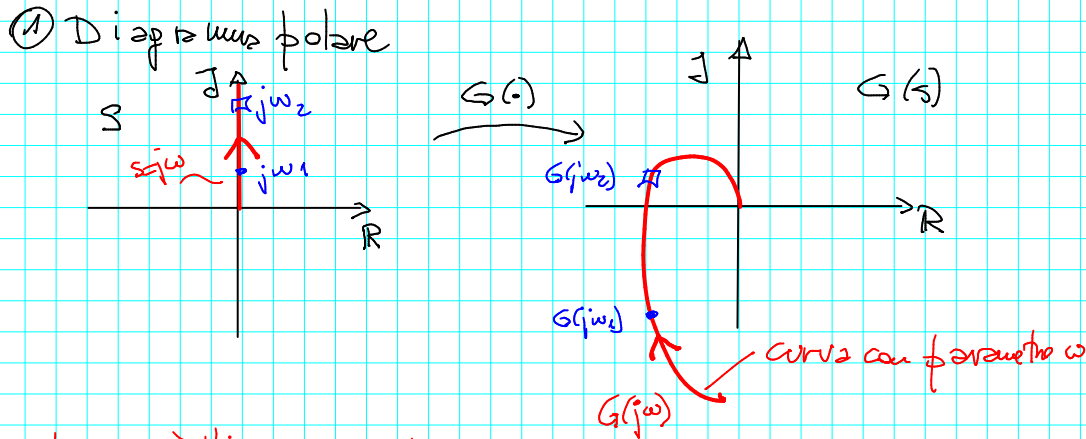
\includegraphics[height=3cm]{../lezione12/img1.PNG}
\end{center}
In un piano immaginario il termine $s = j \omega$ al crescere del valore di $\omega$ cresce lungo l'asse immaginario. Se ora calcoliamo $G(s)$ e lo mostriamo in un secondo piano immaginario, otteniamo una curva $
G(j \omega)$ con parametro $\omega$.\newline
\newline
Possiamo ora dire che la risposta in frequenza è l'immagine attraverso $G$ del semiasse immaginario positivo $J^+$.
\subsection{Diagrammi cartesiani o di Bode}
\subsubsection{Diagramma di Bode del modulo}
[immagine dagli appunti del prof]
\begin{center}
    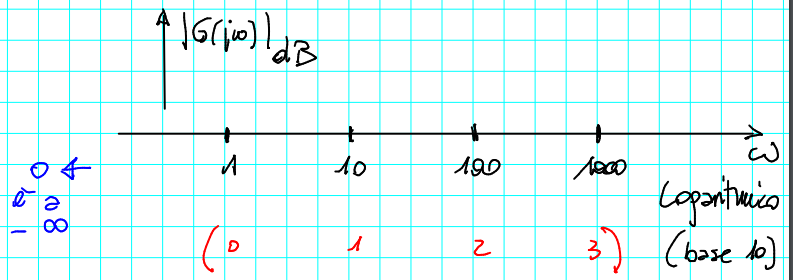
\includegraphics[height=3cm]{../lezione12/img2.PNG}
\end{center}
Il diagramma di Bode del modulo è rappresentato su un piano cartesiano in cui l'asse delle ascisse è l'asse delle $\omega$ e quello delle ordinate è l'asse di $|G(j \omega)|$.\newline
\newline
L'asse delle $\omega$ è logaritmico, cioè a pari distanza non corrisponde pari differenza, ma pari rapporto logaritmico (in base $10$). Inoltre lo zero non viene rappresentato, perchè si trova a $- \infty$, e per questo l'intersezione con l'asse di $|G(j \omega)|$ (cioè l'origine degli assi) non viene rappresentata.\newline
\newline
L'asse di $|G(j \omega)|$ è, invece, espresso in $dB$.\newline
\newline
\textbf{Definizione}: Rappresentare una quantità in $dB$ significa $x_{dB} = 20 log_{10}|x|$.\newline
Per esempio $100_{dB} = 40$; $0,1 _{dB} = -20$; $-0,1 _{dB} = -20$; $1 _{dB} = 0$. Notare che la scrittura in $dB$ non distingue il segno, e inoltre che se $|x| > 1$, allora $x _{dB} >0$ e se $|x|<1$, allora $x _{dB} <0$.
\subsubsection{Diagramma di Bode della fase}
[immagine dagli appunti del prof]
\begin{center}
    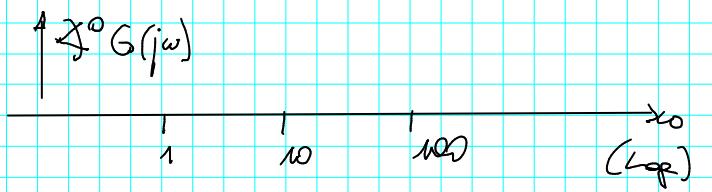
\includegraphics[height=3cm]{../lezione12/img3.PNG}
\end{center}
Anche il diagramma di Bode della fase è rappresentato su un piano cartesiano in cui l'asse delle ascisse è sempre logaritmico ed è l'asse delle $\omega$, invece l'asse delle ordinate è l'asse di $arg(G(j \omega))$ misurato in gradi.
\subsection{Tracciamento dei diagrammi di Bode (asintotici)}
\subsubsection{Forma della funzione di trasferimento per diagrammi di Bode}
Scriviamo la funzione di trasferimento $G(s)$ della cui risposta in frequenza vogliamo i diagrammi di Bode nella forma 
\[
    G(s) = \frac{\mu}{s^g} \cdot \frac{(1 + s \tau_1)(1 + s \tau_2)\dots}{(1 + s t_1)(1 + s t_2)\dots} \cdot \frac{(1 + 2 \frac{\zeta}{\sigma_n}s + \frac{1}{\sigma_n^2}s^2)\dots}{(1 + 2 \frac{\xi}{\omega_n} s + \frac{1}{\omega_n^2}s^2)\dots}
\]
In cui:
\begin{itemize}
    \item prima frazione: il numero $g$ è il \textbf{tipo} della funzione di trasferimento e rappresenta il numero di poli in $s=0$ meno il numero di zeri in $s=0$, o, per dirlo in altri termini, il numero di poli (se positivo) o zeri (se negativo) in $s=0$.\newline
    Per esempio una funzione di trasferimento di tipo $1$ ha un polo nell'origine, una funzione di trasferimento di tipo $-1$ ha uno zero nell'origine, una funzione di trasferimento di tipo $2$ ha due poli nell'origine, una funzione di trasferimento di tipo $0$ non ha nè poli nè zeri nell'origine, etc.
    \item seconda frazione: i vari termini a numeratore del tipo $(1 + s \tau_i)$ rendono conto degli zeri reali non nell'origine; invece i vari termini a denominatore del tipo $(1 + s t_k)$ rendono conto dei poli reali non nell'origine.
    \item terza frazione: infine ci possono essere coppie di zeri complessi coniugati e coppie di poli complessi coniugati, rappresentate dai termini $(1 + 2 \frac{\zeta}{\sigma_n}s + \frac{1}{\sigma_n^2}s^2)$ (per gli zeri) e $(1 + 2 \frac{\xi}{\omega_n} s + \frac{1}{\omega_n^2}s^2)$ (per i poli).
\end{itemize}
Inoltre il numero $\mu$ è detto \textbf{guadagno} della funzione di trasferimento, i termini $t, \tau$ sono \textbf{costanti di tempo} di zeri e poli,  $\omega, \sigma$ si dicono \textbf{frequenze naturali} (o pulsazioni naturali) e $\zeta, \xi$ sono i \textbf{fattori di smorzamento}.\newline
\newline
Una delle proprietà più particolari è che tutto il termine $\frac{(1 + s \tau_1)(1 + s \tau_2)\dots}{(1 + s t_1)(1 + s t_2)\dots} \cdot \frac{(1 + 2 \frac{\zeta}{\sigma_n}s + \frac{1}{\sigma_n^2}s^2)\dots}{(1 + 2 \frac{\xi}{\omega_n} s + \frac{1}{\omega_n^2}s^2)\dots}$ tende a $\rightarrow  1$ per $s \rightarrow 0$, quindi $G(s) \sim \frac{\mu}{s^g}$ per $s \rightarrow  0$.\newline
\newline
\textbf{es.} $G(s) = \frac{(s+2)(s^2-3s+2)}{s^3 + 4 s^2 + s}$.\newline
Trasformiamola nella forma che vogliamo avere per il diagramma di Bode:
\[
    G(s) = \frac{2(1+\frac{s}{2})(s-1)(s-2)}{s(s^2+4s+1)} = \frac{2(1+ \frac{2}{2})(-1)(1-s)(-2)(1-\frac{s}{2})}{s(s-(-2-\sqrt{3}))(s-(-2+\sqrt{3}))}=
\]
\[
    = \frac{2(-1)(-2)(1+\frac{s}{2})(1-s)(1-\frac{s}{2})}{(-2-\sqrt{3})(-2+\sqrt{3})s(1-\frac{s}{-2-\sqrt{3}})(1-\frac{s}{-2+\sqrt{3}})}
\]
in cui $\mu= \frac{2(-1)(-2)}{(-2-\sqrt{3})(-2+\sqrt{3})}$ e $g=1$.\newline
\rule{\textwidth}{0,4pt}
\newline
\newline
Quindi ogni funzione di trasferimento razionale fratta si può esprimere come prodotto di termini del tipo 
\[
    \begin{matrix}
        G_a(s) = \mu & \;\; & G_c(s) = 1+ s t\\
        G_b(s) = \frac{1}{s^g} & \;\; & G_d(s) = 1 + 2 \frac{\xi}{\omega_n}s + \frac{1}{\omega_n^2}s^2
    \end{matrix}
\]
\ \newline
\newline
Allora detti $G_i$ i fattori che compongono $G$, possiamo dire
\[
    G=\prod G_i \;\; \Longrightarrow \;\; \begin{cases}
        |G| = \prod |G_i| \;\; \Longrightarrow \;\; |G|_{dB} = \sum |G_i|_{dB}\\
        arg(G) = \sum arg(G_i)
    \end{cases}
\]
\subsubsection{Diagrammi di bode di modulo e fase di $G_{a,b,c,d}$}
Vediamo perciò come tracciare i diagrammi di bode del modulo e della fase (asintotici) di $G_{a,b,c,d}$. Una volta fatto questo sarà semplice combinarli per arrivare al tracciamento definitivo di $G$.
\begin{itemize}
    \item $G_a(s) = \mu \rightarrow  G_a(j \omega) = \mu \rightarrow \begin{cases}
        |G_a(j \omega)|_{dB} = 20 log_{10}|\mu|\\
        arg(G_a(j \omega)) = \begin{cases}
            0 \;\;\; & \mu>0\\
            -180^o & \mu<0
        \end{cases}
    \end{cases}$.\newline
    \newline
    [immagine dagli appunti del prof]
    \begin{center}
        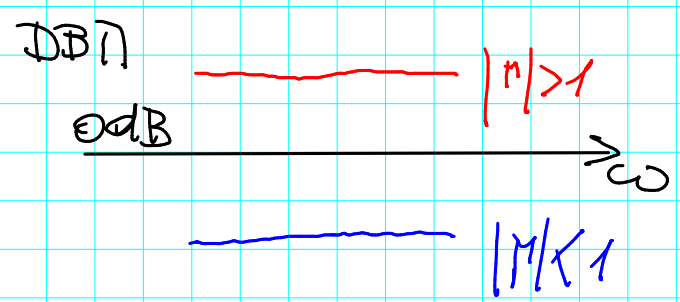
\includegraphics[height=3cm]{../lezione12/img4.PNG}
    \end{center}
    diagramma di bode del modulo: Il diagramma di bode del modulo è una retta orizzontale (se $\mu > 1$ è sopra l'asse delle ascisse, se $\mu < 1$ è sotto l'asse delle ascisse).\newline
    \newline
    [immagine dagli appunti del prof]
    \begin{center}
        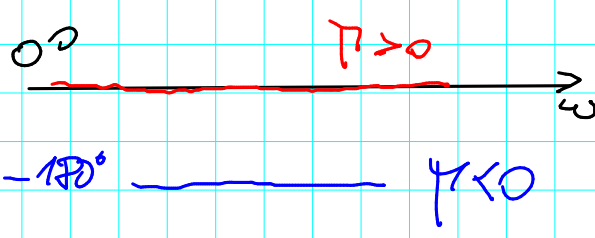
\includegraphics[height=3cm]{../lezione12/img5.PNG}
    \end{center}
    diagramma di bode della fase: Anche il diagramma di bode della fase è una retta orizzontale che coincide con l'asse delle ascisse se $\mu>0$, altrimenti se $\mu<0$ è posta all'altezza di $-180^o$.
\end{itemize}